
\chapter[Metodologia]{Metodologia}
  Esse capítulo irá descrever a metodologia utilizadano desenvolvimento deste trabalho.
Desse modo esse capítulo está dividido nas seções Metodologia de Condução do Trabalho de Conclusão de Curso(\ref{Sec:MetCondTCC}),
Protótipo(\ref{Sec:protótipo}) e Requisitos(\ref{Sec:Requisitos}).
\section{Metodologia de Condução do Trabalho de Conclusão de Curso}
\label{Sec:MetCondTCC}
  Neste capítulo será apresentada a metodologia inicial que foi adotada
para o desenvolvimento deste trabalho.

  Este trabalho foi baseado no exame de qualificação do Roberto \cite{roberto}.
e podemos afirmar que ele pertence a área da engenharia biomédica. "Classicamente,
a Engenharia Biomédica é vista como a aplicação dos métodos de distintas áreas
das Ciências Exatas e de Engenharia no campo das Ciências Médicas e
Biológicas."\cite{engenhariaBiomedica}. Pois ele desenvolve uma abordagem
inovadora aplicado a terapia de  doenças/acidentes motores, neste caso, aplicado a
 fiosioterapia. Onde desenvolve uma nova abordagem para análise de movimentos.

  Para o desenvolvimento deste trabalho, foram necessárias conversas com
o autor para esclarecimento do escopo, da aplicação do trabalho e para a compreensão
do protótipo e seu código fonte, desenvolvido por ele no matlab junto ao exame.
Além disso, faz se necessário o uso da engenharia reversa para identificar os
principais módulos funcionais do protótipo e com isso levantar os requisitos,
que foi por meio de histórias de usuário, então assim desenvolvendo e
implementando as funcionalidades para a familiarização com a tecnologia e o
desenvolvimento do trabalho de conclusão de curso.

   Este trabalho está propondo a criação de um sistema para análise motora,
 para isto é essencial usar uma tecnologia mais difundida e com mais
suporte da comunidade, para esta função foi escolhido o Unity 3d\cite{unity3d} tanto para a interface
humano computador quanto para o processamento, com o auxílio da linguagem C\#.
Para o devido desenvolvimento, necessitou-se de uma fase de aprendizado de ambas
as tecnologias. Os recuros usados foram o manual do Unity 3D \cite{unity3dManual}, a documentação do
C\# \cite{csharpdoc}, além de fóruns online.

\section{Protótipo}
\label{Sec:protótipo}
  Junto com o exame de qualificação citado anteriormente \cite{roberto}, foi
desenvolvido um protótipo no software matlab \cite{matlab}. Esse sistema inicial
implementou algumas das teorias do exame. Ele possui três etapas: rotular os dados,
parametrização e utilizar para segmentação automática.
\begin{itemize}

\begin{sloppypar}

\item \textbf{Rotulação}: Na etapa de rotular os dados,começando pelo arquivo
' SCRIPT\_labelAndIndexMultivariateFile\_WBM21.m '. Neste script estão duas funções,
\textit{labelAndIndexUnivariateFile} que por sua vez chama a função
\textit{labelAndIndexUnivariateStructDataset} que chama a função \textit{labelAndIndexUnivariateDataset}
e \textit{transitionIndexMultivariateFile}.Os dados de entrada são puxados dos arquivos da pasta
'PreProcessedData','/',DecRateN\_Filter,'/',Movement,'/',Subject,'/',Trial,'.mat'.
Esses dados foram coletados previamente por sensores. Os dados são uma struct .mat
com  os ângulos de algumas articulações e o tempo. Esses ângulos são dados em radianos
 e são divididos em articulações e em uma única coluna como podemos observar em \ref{structMatlab}.

\begin{figure}[!h]
\centering
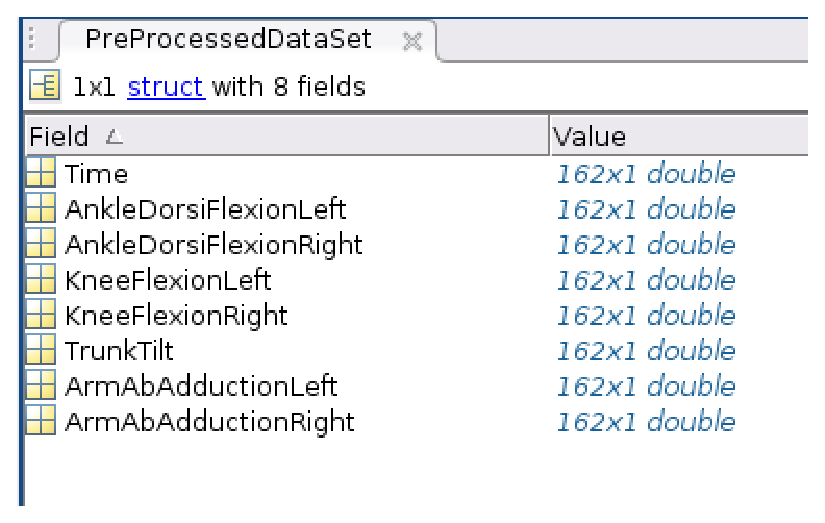
\includegraphics [keepaspectratio=true,scale=0.60]{figuras/structMatlab.eps}
\caption{Dados das articulações}
\label{structMatlab}
\end{figure}

  Quando o script é executado  primeiro um gráfico é traçado com várias curvas
 para selecionar o início e fim de cada conjunto de dados,
depois cada curva é apresentada separadamente. Essa é a etapa para rotular os
dados de cada curva. No prompt ele pergunta qual o “\textit{Switch Variable}”, em seguida
 ele pede para marcar  o início e o fim do intervalo com esse rótulo. A seguir
pergunta se é o fim do  conjunto de dados. Caso não seja o fim ele volta a
 perguntar qual a “Switch Variable”. Esse procedimento se repete para todas as curvas.
Logo após, vem a parte que rotula os dados multivariáveis dependendo do conjunto
de rótulos de cada variável separada. O resultado é a struct “thisLabeledIndexStructDataSet” salvo na pasta
LabeledDataMultivariate’/‘,DecRateN\_Filter,'/',Movement,'/',Subject,'/',Trial,'.mat'.

\item \textbf{Parametrização}: Na etapa de parametrização do modelo a função:
 \"SLDS\_Univariate\_ParameterDataSetBuilder2.m\" pega os dados rotulados da etapa
anterior, ou seja os dados segmentados automaticamente e com as funções
“parametersCteVelSpaceStateModel2” e “hmmTransitionMatrix2” calcula os parâmetros
do Modelo Oculto de Markov. Esta função é a base para o script
"SLDS\_Univariate\_IntraSubject\_ParameterDataset\_Script.m”  que pega diversos
 conjuntos de dados rotulados, de diferentes sujeitos ou diferentes execuções
do mesmo sujeito e chama a função “SLDS\_Univariate\_ParameterDataSetBuilder2.m”
 para cada um deles e no fim temos os parâmetros do modelo oculto de Markov ajustado
 para vários conjuntos de treinamento.

\end{sloppypar}
\item \textbf{Segmentação}: Esse é o programa que faz a estimação dos rótulos associado com cada medida.
A principal função é a “SLDS\_Filter\_Univariate” ela recebe as structs
ValidationTrialThisVariable e FittedModelThisVariable e a variável
InitialSwitchVariableState. A ValidationTrialThisVariable contém os dados a serem
 classificados e pode conter também os rótulos. São as medidas do movimento, os
mesmos dados usados na parte de rotulação. O FittedModelThisVariable são todos
os parâmetros do modelo (análogo aos parâmetros do ModeloOculto de Markov).
A variável InitialSwitchVariableState indica o símbolo da primeira medida.

Na imagem \ref{diagramProt} podemos ver todo o fluxo de dados do protótipo.
\end{itemize}

\begin{figure}[!h]
\centering
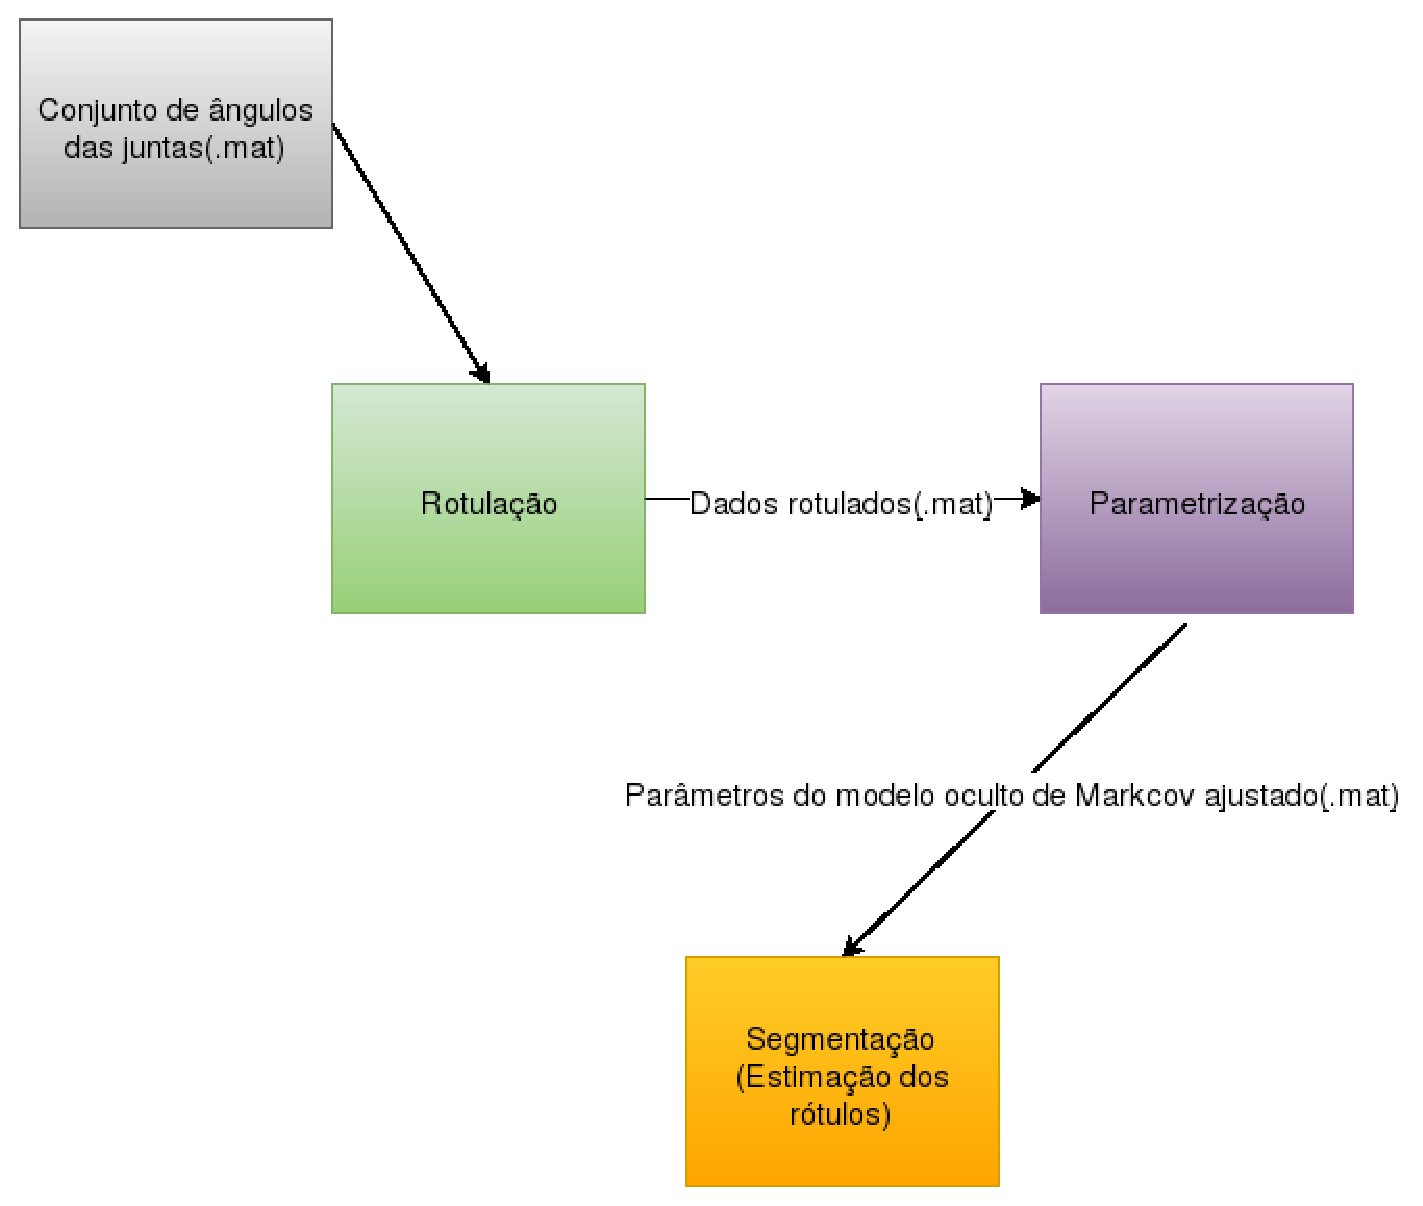
\includegraphics [keepaspectratio=true,scale=0.60]{figuras/diagramProt.eps}
\caption{Fluxo de Dados}
\label{diagramProt}

\end{figure}


\section {Requisitos}
\label{Sec:Requisitos}
  Um requisito é definido como "uma condição ou uma capacidade com a qual o
sistema deve estar de acordo"\cite{requisitos}. Existem vários tipos de
requisitos. Um modo de categorizá-los é descrito como o modelo
FURPS+\cite{robertGrady} , seguindo esse modelo, elicitamos os requisitos
iniciais do sistema:
  \begin{itemize}
  \item \textbf{Funcionalidade}(Functionality):
    \begin{itemize}
    \item Software para auxilar o acompanhamento de pacientes em reabilitação
    motora de movimentos específicos.
    \item É realizado por meio de comparação do movimento das articulações do
     corpo humano em tempo real, com uma base de articulações com os movimentos
    previamente estabelicidos.
    \item Apresenta um conjunto de movimentos gravados para seleção e execução.
    \end{itemize}
  \item \textbf{Usabilidade}(Usability)
    \begin{itemize}
    \item O usuário do sistema será capaz de visualizar todo tipo de informação
     textual, imagem ou modelo 3d na aplicação , com clareza, em qualquer
    monitor independente de resolução.
    %\item Documentação ampla e de fácil compreensão, abordando todas as
    %funcionalidades disponível na aplicação.
    \end{itemize}
\item \textbf{Confiabilidade}(Reability)
    \begin{itemize}
    \item O sistema será capaz de verificar algum erro ou inconstância entre os
     dados recebidos dos sensores, podendo assim se recuperar ou informar
    alguma falha na comunicação com os mesmos.
    \end{itemize}
\item \textbf{Desempenho}(Performance)
    \begin{itemize}
    \item O sistema analisará o movimento feito pelo usuário em tempo real.
    \end{itemize}
\item \textbf{Suportabilidade}(Supportability)
    \begin{itemize}
    \item Em sua versão inicial será exclusivo do sistema operacional da microsoft, o windows, podendo ser executado nas versões 7,8 e 10.
    \end{itemize}
  \end{itemize}

\subsection{Funcionalidades do sistema - \textit{features}}\label{sub:features}
    As \textit{features} no desenvolvimento ágil é um pedaço de funcionalidade que oferece valor comercial \cite{versionOne}.
  Geralmente as \textit{features} tem uma granularidade maior que as \textit{User Stories}(Histórias de usuário~\ref{sec:Histórias de usuário}).
  Podemos dizer que algumas features são compostas de \textit{User Stories}.

    O sistema possui três features, gravação de movimento, leitura de arquivo do movimento desejado e análise da repetição do movimento:
  \begin{enumerate}
    \item \textbf{Gravar movimento:} Essa funcionalidade permite a gravação do movimento, deve ser feito pelo profissional fisioterapeuta
    para uma correta execução. Será esse movimento que o sistema usará como gabarito. O sistema retorna um arquivo csv.
    \item \textbf{Ler arquivo de movimento:} Essa funcionalidade espera um arquivo csv e armazena o movimento no sistema.
    \item \textbf{Praticar movimento:} Essa funcionalidade mostra a correta execução do movimento e analisa com o movimento do paciente.
  \end{enumerate}

  Podemos ver o detalhamento das features em Histórias de usuário do sistema(\ref{historias}).
\subsection{Histórias de usuário do sistema}
\label{sec:Histórias de usuário}
  Como prática ágil as \textit{User stories}(Histórias de usuário), são artefatos
de desenvolvimento, utilizadas para organizar requisitos. Tem-se foco nos objetivos
do usuário e como o sistema alcança esses objetivos.

  Para melhor organizar e fracionar os requisitos deste trabalho, foi adotado
essa prática ágil, podemos ver o levantamento das histórias de usuário na tabela Histórias(\ref{historias}).
\begin{table}[H]
\centering
\caption{Histórias}
\label{historias}
\begin{tabular}{|l|l|}
\hline
\textbf{História} & 1                                                        \\ \hline
\textbf{Eu como}  & Fisioterapeuta                    \\ \hline
\textbf{Desejo}   & Que o sistema mapeie meu movimento sendo executado corretatmente                   \\ \hline
\textbf{Para}     & poder comparar com o movimento do paciente \\ \hline
 \multicolumn{2}{|l|}{}                                                       \\ \hline
\textbf{História} & 2                                                        \\ \hline
\textbf{Eu como}  & Usuário                                    \\ \hline
\textbf{Desejo}   & Poder carregar movimento previamente mapeado                \\ \hline
\textbf{Para}     & Constar no menu do sistema\\ \hline
\multicolumn{2}{|l|}{}                                                       \\ \hline
\textbf{História} & 3                                                        \\ \hline
\textbf{Eu como}  & Fisioterapeuta                    \\ \hline
\textbf{Desejo}   & Que o sistema salve um novo movimento                    \\ \hline
\textbf{Para}     & Poder constar no menu do sistema e poder ser executado \\ \hline
\multicolumn{2}{|l|}{}                                                       \\ \hline
\textbf{História} & 4                                                        \\ \hline
\textbf{Eu como}  & Usuário                                                  \\ \hline
\textbf{Desejo}   & Desejo escolher movimento de referência                  \\ \hline
\textbf{Para}     & Melhor seguir receita médica                             \\ \hline
\multicolumn{2}{|l|}{}                                                       \\ \hline

\textbf{História} & 5                                                        \\ \hline
\textbf{Eu como}  & Usuário                                                  \\ \hline
\textbf{Desejo}   & Feedback do movimento sendo executado em tempo real                    \\ \hline
\textbf{Para}     & Poder melhor executar os movimentos das articulações           \\ \hline
\multicolumn{2}{|l|}{}                                                       \\ \hline

\end{tabular}
\end{table}

  Tais histórias compões as funcionalidades do sistema(\ref{sub:features}) e foram implementadas no Unity 3d.

\section{Metodologia Adotada no Desenvolvimento da Ferramenta}
  Iremos adotar algumas práticas ágeis e o \textit{kanban}\cite{kanban}
 para gerenciamento.Nesta seção iremos descrever tais práticas,
além dos papéis envolvidos.

  Para o \textit{Product Backlog} e \textit{kanban}  usaremos a ferramenta trello. Trello é uma ferramenta
\textit{e-kanban}\cite{kanban} e que facilita o gerenciamento de projetos, que pode ser ajustada de acordo com as necessidades
do usuário. O \textit{Product Backlog} estará disponível inicialmente somente para
os envolvidos neste trabalho.

  As \textit{Sprints} terão duração de duas semanas. Já as \textit{Sprints Plannings}
e as \textit{Sprints reviews}, terão durações de no máximo uma hora e serão
discutidas com os responsáveis por desempenhar os papéis de \textit{Product Owner}.


\subsection{Arquitetura do sistema}
\label{Sec:arquitetura}
  De acordo com a ISO/IEEE 1471-2000 - Arquitetura é a organização fundamental
de um sistema incorporada em seus componentes, seus relacionamentos com o
ambiente, e os princípios que conduzem seu design e evolução.

  A arquitetura será mais detalhada no capítulo Proposta(\ref{ch:proposta}) na seção Arquitetura(\ref{sub:arquitetura}).

\subsection{Planejamento das atividades}
\label{Sec:Planejamento}
  Esta seção, descreve um cronograma de todas atividades
. Cronograma  é uma representação de um plano de
execução das atividades do trabalho, incluindo  outras
informações de planejamento.

O TCC, segundo as regras da UnB, é realizado em duas fases: uma chamada de TCC\_01 e outra chamada de TCC\_02.
 Durante o TCC\_01, o foco desse trabalho foi estabelecer os pilares teóricos para embasamento do projeto como um todo.
 Já durante o TCC\_02, o trabalho estará focado desenvolver um sistema para análise motora, atingindo uma prova de conceito,
  visando a viabilidade da proposta, com base nas fundamentações teóricas - conquistados ao longo do TCC\_01.

O TCC\_01 pôde ser sub-dividido em sete atividades: \textit{selecionar tema}, \textit{realizar pesquisa bibliográfica},
 \textit{definir proposta}, \textit{escrever referencial teórico}, \textit{estabelecer suporte tecnológico},
  \textit{evoluir metodologia} e \textit{apresentar TCC 1}.
  As mesmas estão distribuídas de acordo com o cronograma disposto na Tabela \ref{tab:cronograma1}.

\begin{table}[H]
	\centering
	\caption{Cronograma de atividades TCC\_1.}
	\label{tab:cronograma1}
	\begin{tabular}{@{}ccccc@{}}
		\toprule
		\textbf{Cronograma}             & \textbf{Março} & \textbf{Abril} & \textbf{Maio} & \textbf{Junho} \\ \midrule
		Selecionar Tema                 & X              &                &               &                \\ \midrule
		Realizar pesquisa bibliográfica & X              & X              & X             & X              \\ \midrule
		Definir proposta                & X              &                &               &                \\ \midrule
		Escrever referencial teórico    &                & X              & X             &                \\ \midrule
		Estabelecer suporte tecnológico &                & X              & X             & X              \\ \midrule
		Evoluir metodologia             &                & X              & X             &                \\ \midrule
		Apresentar TCC 1                &                &                &               & X              \\ \bottomrule
	\end{tabular}
\end{table}

Já a segunda etapa do trabalho, durante a realização do TCC\_2, o cronograma de atividades segue o apresentado na Tabela \ref{tab:cronograma2}.

\begin{table}[H]
	\centering
	\caption{Cronograma de atividades TCC\_2.}
	\label{tab:cronograma2}
	\begin{tabular}{@{}cccccc@{}}
		\hline
		\textbf{Cronograma}                                                           & \textbf{Março} & \textbf{Abril} & \textbf{Maio} & \textbf{Junho} & \textbf{Julho} \\ \hline
		\begin{tabular}[c]{@{}c@{}}Configurar\\Kinect/PC e ambiente\end{tabular}      & X               & X                          &                  &                   &                   \\ \hline
		Desenvolver solução \ref{historias}                                            &                 & X                          & X                & X                 &                   \\ \hline
		Testar solução                                                                &                 & X                          & X                & X                 &                   \\ \hline
		Analisar resultados                                                           &                 &                            &                  & X                 & X                 \\ \hline
		Apresentar TCC\_2                                                           &                 &                            &                  &                  & X                 \\ \hline
	\end{tabular}
\end{table}

\begin{itemize}
	\item \textbf{Propor tema}:

		A atividade de propor tema engloba desde a escolha do contexto em que se deseja trabalhar, até a definição dos orientadores do trabalho. Após a escolha do contexto e dos orientadores, buscou-se definir um escopo que será abordado durante o trabalho, ou seja, o tema. Os orientadores devem validar o tema escolhido para concluir a atividade.

	\item \textbf{Levantar bibliografia base}:

		Esta atividade refere-se à definição de pilares para o estudo proposto, ou seja, estabelecer o marco teórico do trabalho. Este levantamento garante o entendimento do contexto trabalhado e as possibilidades de atuação, especificando mais adequadamente o escopo.

	\item \textbf{Definir proposta}:

		Documentar a proposta de pesquisa para este trabalho. A proposta inclui, não apenas, mas, principalmente, uma introdução com a contextualização do tema, o objetivo geral e específicos, a justificativa e uma metodologia de pesquisa.

	\item \textbf{Realizar pesquisa e análise bibliográfica}:

		A pesquisa bibliográfica foi feita a partir do exame de qualificação do Roberto \cite{roberto}

	\item \textbf{Realizar referencial teórico}:

		O mesmo descreve o referencial teórico do trabalho em andamento.

	\item \textbf{Estabelecer suporte tecnológico}:

		Nesta atividade, são definidas as principais ferramentas e tecnologias utilizadas para a execução deste trabalho.

	\item \textbf{Apresentar TCC\_1}:

		Apresentar os resultados obtidos até o momento para a banca examinadora.

  \item \textbf{Desenvolver solução}:

    Desenvolvimento das histórias de usuário\ref{historias} levantandas ao longo do TCC\_1.

  \item \textbf{Testar solução}:

    Esta atividade ocorre em sicronia com a atividade de desenvolvimento, é essencial para analisar acordo com as histórias de usuário.

  \item \textbf{Analisar resultados}:

    Registrar e analisar informações relevantes que foram obtidas ao longo do desenvolvimento.

  \item \textbf{Apresentar TCC\_2}:

    Apresentar os resultados obtidos para a banca examinadora.
\end{itemize}
